% The MIT License (MIT)
% =====================

% **Copyright (c) 2018 Anish Athalye (me@anishathalye.com)**

% Permission is hereby granted, free of charge, to any person obtaining a copy of
% this software and associated documentation files (the "Software"), to deal in
% the Software without restriction, including without limitation the rights to
% use, copy, modify, merge, publish, distribute, sublicense, and/or sell copies
% of the Software, and to permit persons to whom the Software is furnished to do
% so, subject to the following conditions:

% The above copyright notice and this permission notice shall be included in all
% copies or substantial portions of the Software.

% THE SOFTWARE IS PROVIDED "AS IS", WITHOUT WARRANTY OF ANY KIND, EXPRESS OR
% IMPLIED, INCLUDING BUT NOT LIMITED TO THE WARRANTIES OF MERCHANTABILITY,
% FITNESS FOR A PARTICULAR PURPOSE AND NONINFRINGEMENT. IN NO EVENT SHALL THE
% AUTHORS OR COPYRIGHT HOLDERS BE LIABLE FOR ANY CLAIM, DAMAGES OR OTHER
% LIABILITY, WHETHER IN AN ACTION OF CONTRACT, TORT OR OTHERWISE, ARISING FROM,
% OUT OF OR IN CONNECTION WITH THE SOFTWARE OR THE USE OR OTHER DEALINGS IN THE
% SOFTWARE.


% Gemini theme
% https://github.com/anishathalye/gemini

\documentclass[final]{beamer}

% ====================
% Packages
% ====================

\usepackage[T1]{fontenc}
\usepackage{lmodern}
\usepackage[size=custom,width=130 ,height=100,scale=1.0]{beamerposter}
\usetheme{gemini}
\usecolortheme{gemini}
\usepackage{graphicx}
\usepackage{booktabs}
\usepackage{tikz}
\usepackage{pgfplots}
\usepackage{tcolorbox}
\usepackage{geometry}

% ====================
% Lengths
% ====================

% If you have N columns, choose \sepwidth and \colwidth such that
% (N+1)*\sepwidth + N*\colwidth = \paperwidth
\newlength{\sepwidth}
\newlength{\colwidth}
\setlength{\sepwidth}{0.025\paperwidth}
\setlength{\colwidth}{0.3\paperwidth}

\newcommand{\separatorcolumn}{\begin{column}{\sepwidth}\end{column}}

% ====================
% Title
% ====================

\title{Developing a QIIME 2 plugin - a Simple Annotation for Robust Tools}

\author{Christopher R. Keefe \and Evan Bolyen \textsuperscript{†} \and Matthew Ryan Dillon \textsuperscript{†} \and J. Gregory Caporaso \textsuperscript{†} }

\institute[shortinst]{The Pathogen and Microbiome Institute at Northern Arizona University \\
{\footnotesize \textsuperscript{†} Advisors} }

% ====================
% Body
% ====================

\begin{document}

\begin{frame}[t]
\begin{columns}[t]
\separatorcolumn

\begin{column}{\colwidth}

  \begin{block}{Objective and Introduction}

    \textbf{Objective:} To provide a high-level introduction to the process and
     benefits of developing a  QIIME 2 \cite{10.7287/peerj.preprints.27295v1}
     plugin for computational methods for microbiome science.
    \hfill\break

    \textbf{Introduction:} By wrapping a script in a python 3 package, then
    annotating it with information about the commands it makes available, the
    parameters they expose, and the types of data they take in and put out, a
    plugin author can take advantage of existing QIIME 2 infrastructure. This
    can greatly increase the robustness and accessibility of their script,
    improve distribution and citation, and facilitate the integration of
    their method with new and existing analytical pipelines.
    \hfill\break

    \textbf{QIIME 2 provides:}
    \begin{itemize}
      \item \textbf{Interfaces:} Familiar user interfaces for a diverse
      user base (e.g. CLI, API, GUI, galaxy, cwl)
      \item \textbf{Community:} A vibrant user base, free forum infrastructure for
      plugin support
      \item \textbf{Visibility:} Centralized plugin publishing through the QIIME 2
      Library
      \item \textbf{Provenance:} Integrated and automatic tracking of data provenance,
      and built-in citation support
      \item \textbf{Low-level infrastructure:} Facilitates data I/O, communication
      between disparate methods in an analytical pipeline, and cross-platform compatability
      \item \textbf{Semantic typing:} A rich and extensible type system prevents user
      error, supports backwards compatability and collaboration
      \item \textbf{Sharing:} Allows secure interaction with QIIME 2 Results
       without a software installation
    \end{itemize}
  \end{block}

  \begin{figure}[tph!]
  {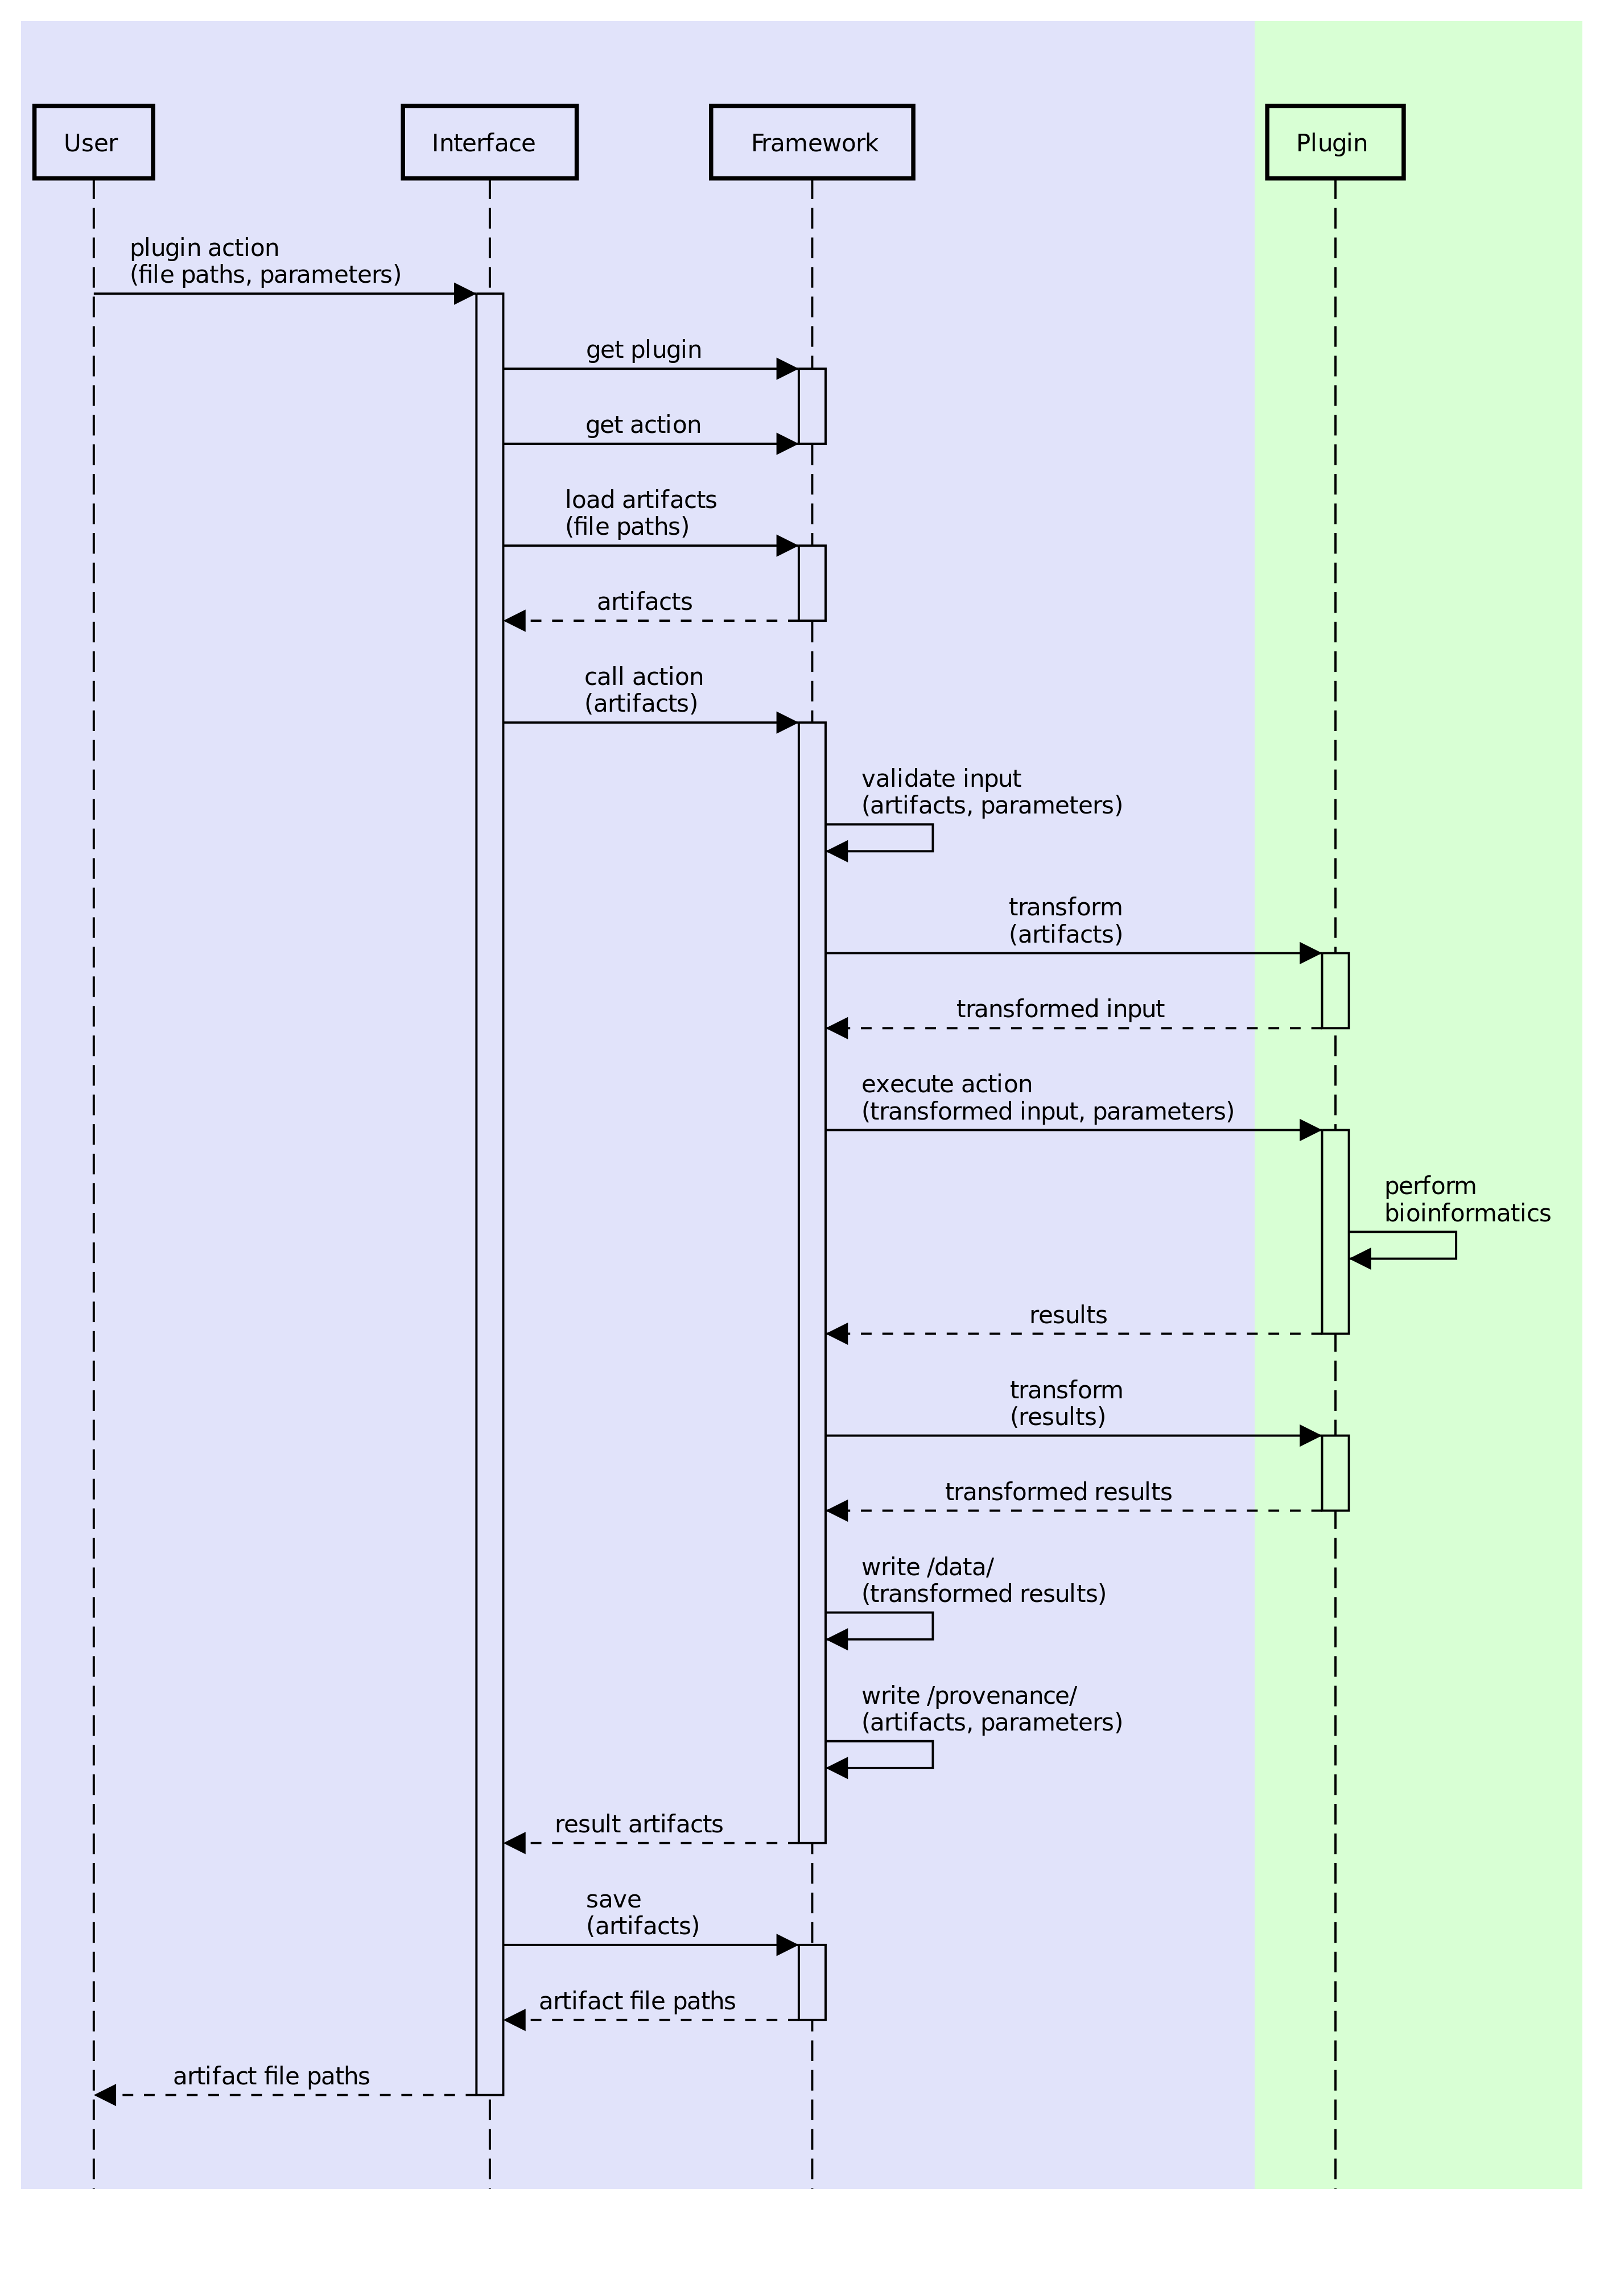
\includegraphics[height=20cm]{assets/action_call_sequence_diagram}}
  \caption{\,Plugins (green) reduce development overhead by utilizing existing infrastructure (blue).}
  \label{fig:callSequence}
  \end{figure}

  \begin{block}{Develop a method or algorithm}

  In order to develop a QIIME 2 plugin, you must first have code you would
  like to run in QIIME 2. Your method may be written Python 3, or in any
  language accessible to Python 3 with a sub-process call: popular plugins wrap
  code written in R and C, and many options exist.\\
  \hfill\break
  Example: the q2\_alignment plugin wraps the MAFFT application by importing \code{subprocess}, generating I/O filepaths, building a command for the OS, and using that command to run MAFFT.\\
      \begin{tcolorbox}
    [width=\textwidth, colframe=blue]
      {
{\texttt{\textcolor{codeblack}{
import subprocess\\
from q2\_types.feature\_data import DNAFASTAFormat, AlignedDNAFASTAFormat\\
\begin{tabbing}
def \=maff\=t(se\=quences: DNAFASTAFormat,\\
\>\>n\_threads: int = 1,\\
\>\>parttree: bool = False) -> AlignedDNAFASTAFormat:\\
\>unaligned\_filepath = str(sequences.path)\\
\>result = AlignedDNAFASTAFormat()\\
\>aligned\_filepath = str(result.path)\\
\\
\>cmd = ["\=mafft", "--preservecase", "--inputorder",\\
\>\>\>"--thread", str(n\_threads), unaligned\_filepath]\\
\\
\>with open(aligned\_filepath, 'w') as output\_f:\\
\>\>subprocess.run(cmd, stdout=output\_f, check=True)
\end{tabbing}}}}
      }
    \end{tcolorbox}
  \end{block}

  \begin{block}{Introduce new kinds of data}
    Some computational methods require the creation of novel data formats, or
    entirely new types of data. By defining these as Semantic Types in your plugin,
    you allow other QIIME 2 plugins to recognize and use your new data types effectively.

    \begin{tcolorbox}
    [width=\textwidth, colframe=blue]
    {NOTE: The creation of new Semantic Types is a great opportunity for collaboration
    with other developers in the field. Well-architected Types benefit analytical pipeline
    development, and help improve QIIME 2's "understanding" of microbiome data. Further,
    a clear understanding of the Types your method interacts with can clarify and improve the method
    development process.}
    \end{tcolorbox}
  \end{block}

\end{column}

\separatorcolumn

\begin{column}{\colwidth}

\begin{block}{Annotate your method}
  Plugin annotation allows the QIIME 2 framework to recognize and communicate with plugins.
  Further, it creates a "common language" for composing analytical pipelines,
  assigning semantic types to method results which allow them to be interpreted by other
  methods in any other plugin.

  Plugin annotation is simple (see Figure ~\ref{fig:registrationDiagram}), and allows plugin documentation
  to be generated in any interface. Citation information registered in plugins
  is automatically captured in Result provenance.

  To annotate your plugin:

  \begin{enumerate}
    \item Import any necessary dependencies (e.g. the \code{Plugin}) method from \code{qiime2.plugin},
    or existing semantic types from \code{q2\_types}), and the top-level folder that holds your plugin's methods. TODO: WORKSHOP THIS
    \item Use \code{Plugin()} to register your plugin.
    \item Use \code{register\_function()} to register \textit{each} public method the plugin offers
    \item Use \code{TODO: FX Name} to register any new semantic types or formats available in this plugin.
  \end{enumerate}

\end{block}

  \begin{block}{Visualizations}
    \begin{figure}[tph!]
    {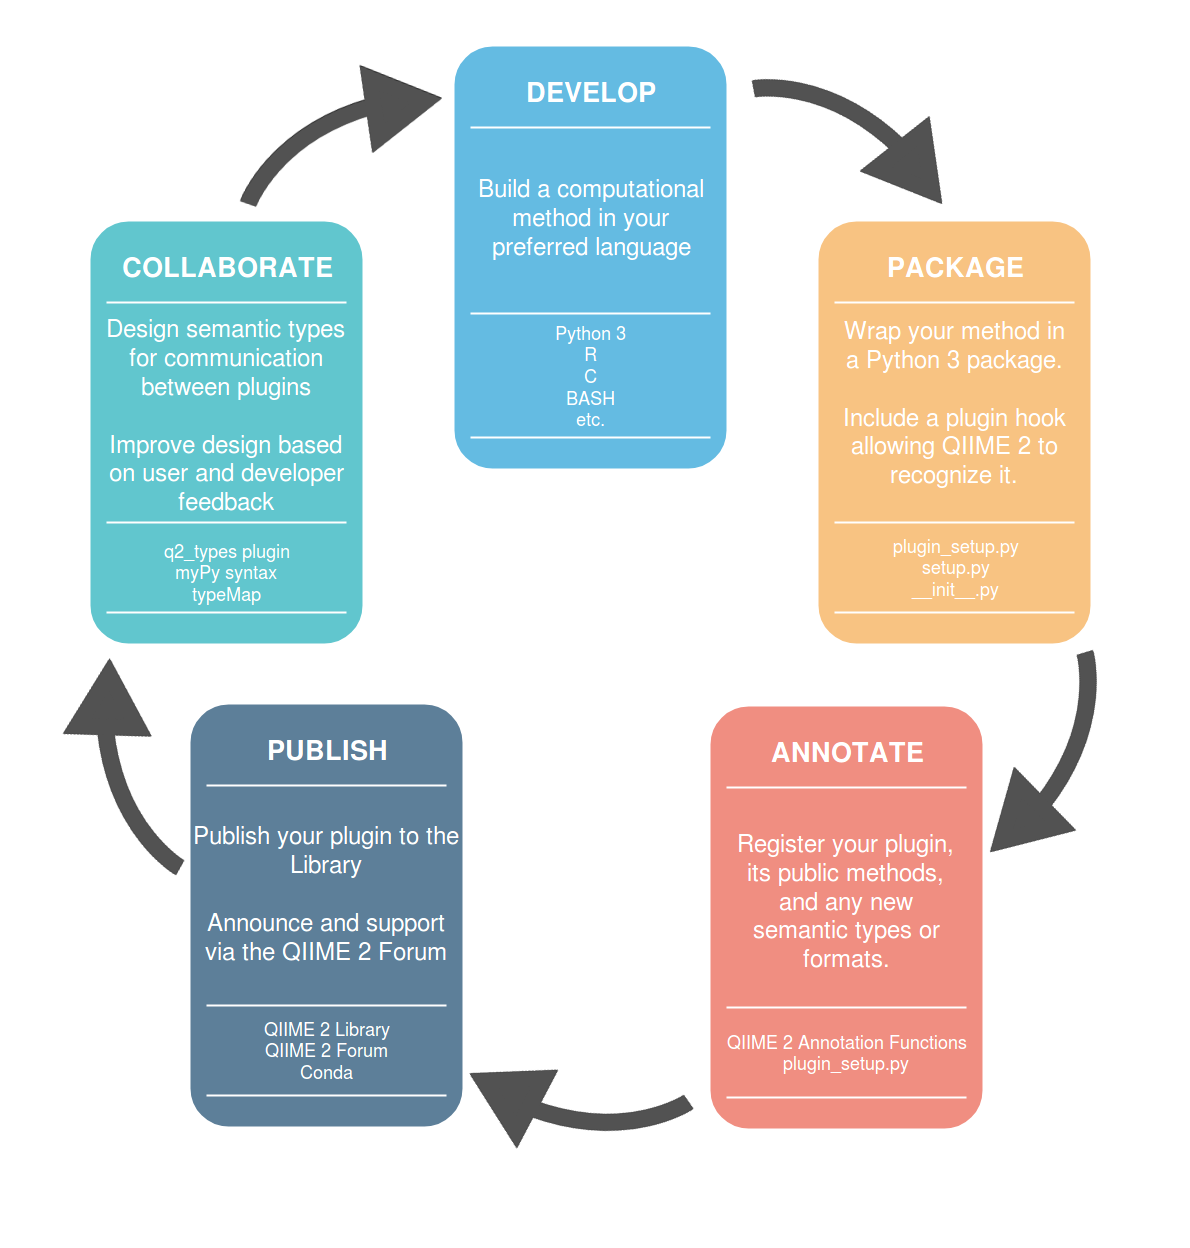
\includegraphics[height=24cm]{assets/DevelopmentProcessDiagramGreyWBG}}
    \caption{\,QIIME 2 plugin development cycle diagram. }
    \label{fig:processDiagram}
    \end{figure}

    \begin{figure}[tph!]
    {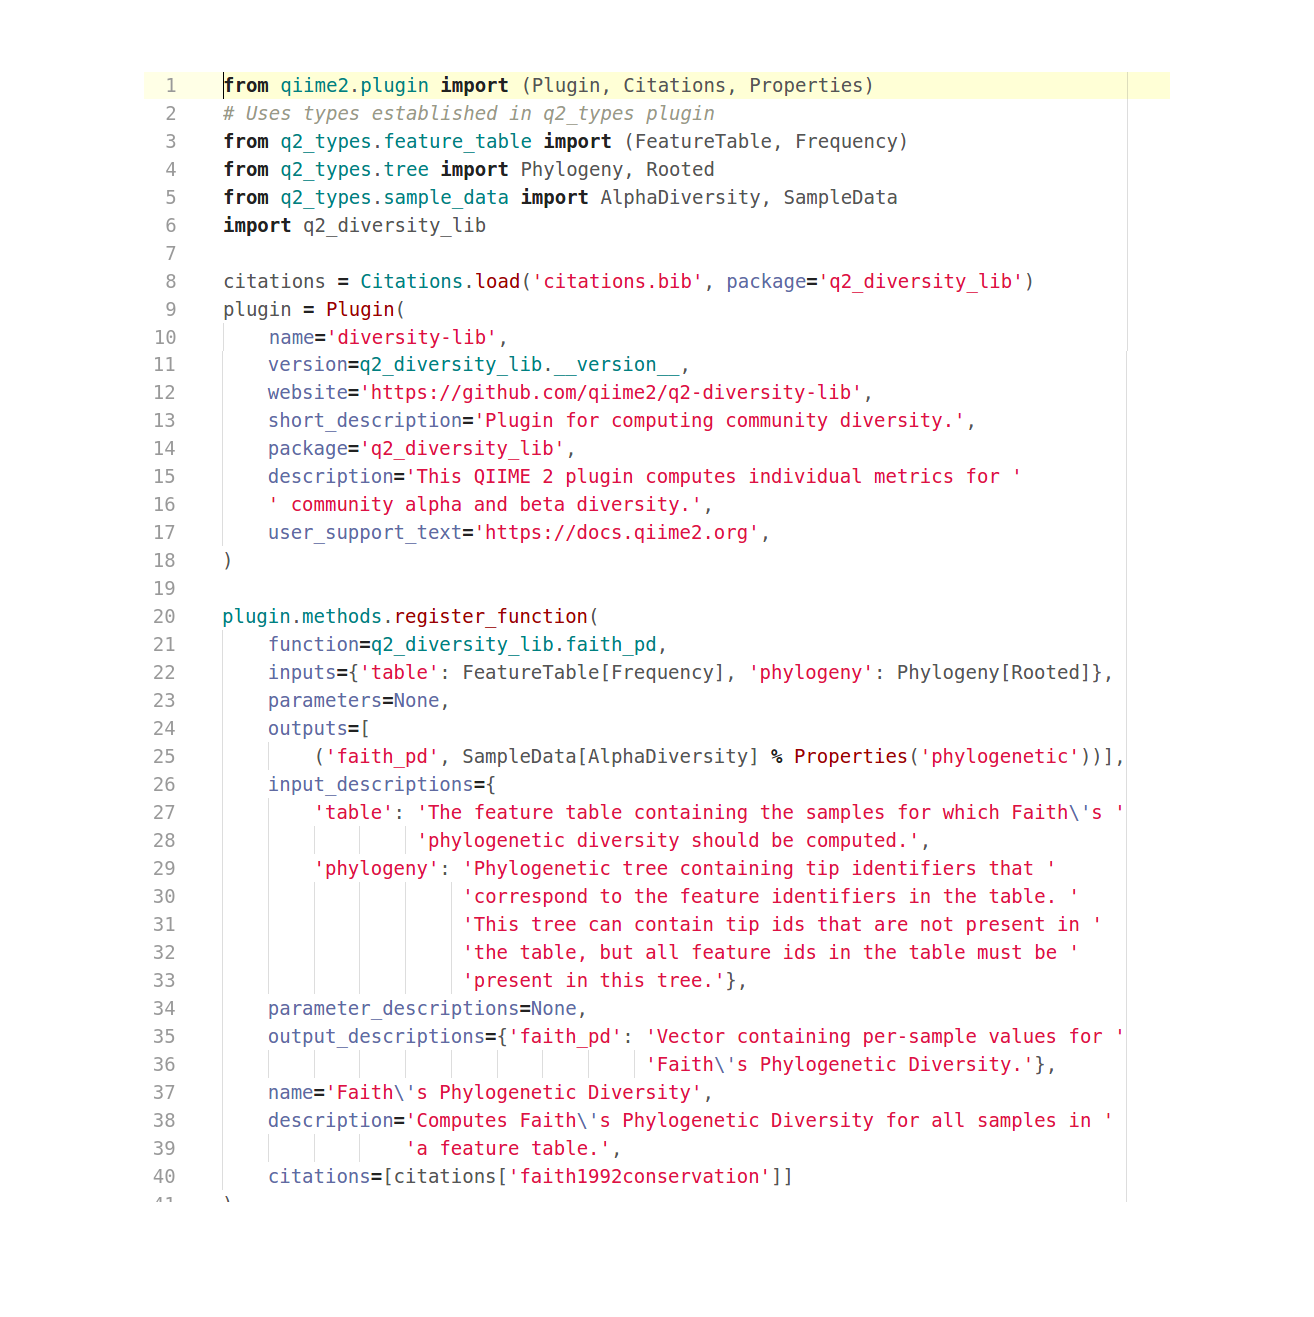
\includegraphics[height=24cm]{assets/registrationDiagram}}
    \caption{\,Overview of registration annotation for QIIME 2 plugins}
    \label{fig:registrationDiagram}
    \end{figure}

  \end{block}

  \begin{block}{Project Funding}
      \begin{figure}[!htb]
        \minipage{0.31\textwidth}%
          \begin{center}
            
\includegraphics[width=.35\linewidth]{assets/SponsorLogos/ABOR}
          \end{center}
        \endminipage
        \hskip 2cm
        \minipage{0.31\textwidth}
          \begin{center}
            
\includegraphics[width=.42\linewidth]{assets/SponsorLogos/APSloanFdn}
          \end{center}
        \endminipage\hfill
        \minipage{0.31\textwidth}
          \begin{center}
            
\includegraphics[width=.50\linewidth]{assets/SponsorLogos/NSF}
          \end{center}
        \endminipage\hfill
      \end{figure}
  \end{block}
\end{column}

\separatorcolumn

\begin{column}{\colwidth}

  \begin{block}{Create a python package}

    Plugins are python packages with metadata hooks QIIME 2 uses to facilitate
    communication with the other plugins in a deployment. Packaging
    simplifies plugin installation for users, and provides access to the QIIME 2 platform.

    \begin{figure}[tph!]
      {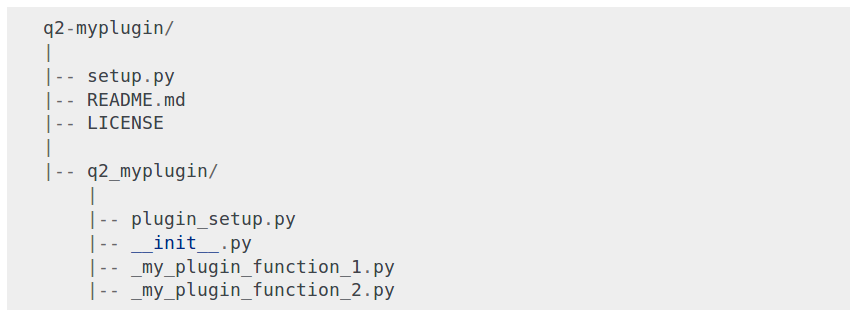
\includegraphics[height=10cm]{assets/package_structure}}
      \caption{\,File map of a simple python package. Note \code{plugin\_setup.py} required for QIIME 2 plugins.
      TODO: Rebuild this in a more visually appealing way.}
      \label{fig:packageStructure}
    \end{figure}

    \begin{tcolorbox}
    [width=\textwidth, colframe=blue]
    {Python packaging may be the most challenging part of plugin creation
    for new developers, because software structure impacts package structure.
    Generally, the structure resembles Figure ~\ref{fig:packageStructure}}
    \end{tcolorbox}

    General guidelines:
    \begin{itemize}
      \item Define one or more Python 3 functions, installable with \code{setuptools}
      \item In your \code{plugin\_setup.py}, instantiate a \code{qiime2.plugin.Plugin} object
      \item In your plugin package's \code{setup.py}, define that instance as an entry point
      \item Include \code{\_\_init\_\_.py} files for every subfolder of your plugin which
      contains function definitions. These make function names accessible for registration and use.
    \end{itemize}
  \end{block}

  \begin{block}{Publish and support}

    Completed plugins may be published to the QIIME 2 Library, and announced
    in the Community Contributions category of the QIIME 2 forum. Many developers
    also use the forum as their primary platform for user support.

    Though optional, most developers publish their plugins on Conda. This greatly
    improves dependency handling and simplifies installation.

  \end{block}

  \begin{block}{Future capabilities}

    \begin{itemize}
      \item \textbf{TODO: SP? Type Map:} A new type map system will launch in QIIME 2 2019.4,
      allowing developers powerful new tools for manipulating and constraining the types of
      data used and produced by methods. Type map will allow plugins to assign
      nuanced types to their outputs programatically (e.g. based on parameterization),
      and will enhance plugins' ability to intelligently constrain allowable data inputs.
    \end{itemize}

  \end{block}

  \begin{block}{Further Reading}
    \begin{itemize}
      \item \href{https://dev.qiime2.org/latest/tutorials/first-plugin-tutorial/}{Developing a (QIIME 2) Plugin for Dummies: dev.qiime2.org/latest/tutorials/first-plugin-tutorial/}
      \item \href{https://docs.qiime2.org/2019.1/plugins/developing/}{Developing a QIIME 2 Plugin: docs.qiime2.org/2019.1/plugins/developing/}
      \item \href{https://dev.qiime2.org/latest/storing-data/types/}{Semantic and Primitive Types: dev.qiime2.org/latest/storing-data/types/}
      \item \href{https://library.qiime2.org/}{QIIME 2 Library: library.qiime2.org/}
      \item \href{https://python-packaging.readthedocs.io/en/latest/minimal.html}{Python Packaging: python-packaging.readthedocs.io/en/latest/minimal.html}
      \item \href{https://dev.qiime2.org/latest/tutorials/conda-tutorial/}{Publishing plugins on Conda: dev.qiime2.org/latest/tutorials/conda-tutorial/}
    \end{itemize}
  \end{block}

  \begin{block}{References}
    \nocite{*}
    \bibliographystyle{acm}\bibliography{poster}
  \end{block}

  \begin{figure}
    \begin{minipage}[c]{\textwidth}
      \hfill
      
\includegraphics[height=5cm]{assets/repo}
    \end{minipage}
    \begin{minipage}[c]{\textwidth}
      \hfill
      Poster Source: https://github.com/ChrisKeefe/SACMDA19
    \end{minipage}
  \end{figure}

\end{column}

\separatorcolumn
\end{columns}
\end{frame}
\end{document}
